\documentclass[prodmode]{acmlarge}

\pdfpagewidth=8.5in
\pdfpageheight=11in

\usepackage{latexsym}
\usepackage{amssymb}
\usepackage{graphicx}
\usepackage{bbding}
\usepackage{pifont}
\usepackage[T1]{fontenc}
\usepackage{pslatex}
\usepackage{url}
%\usepackage{minted}
\usepackage{listings}

\acmVolume{}
\acmNumber{}
\acmArticle{}
\articleSeq{}
\acmYear{2013}
\acmMonth{10}

\markboth{Bijvank et al.}{Software Architecture Patterns for System Administration Support}
\title{Software Architecture Patterns for System Administration Support}
\author{ROLAND BIJVANK \affil{HU University of Applied Sciences, Utrecht, the Netherlands}\ \\
WIEBE WIERSEMA \affil{HU University of Applied Sciences, Utrecht, the Netherlands}\ \\
CHRISTIAN K\"{O}PPE \affil{HAN University of Applied Sciences, Arnhem, the Netherlands}}
%\author{ROLAND BIJVANK , WIEBE WIERSEMA and CHRISTIAN K\"{O}PPE \affil{HU University of Applied Sciences, Utrecht, the Netherlands\\ \{roland.bijvank,wiebe.wiersema,christian.koppe\}@hu.nl}}
\parskip=0.3em

%Peter Sommerlad: Yes Patterns(!)
%No footnotes, but references!
%Intended audience?
%Need more work!
%+Whitespace, diagrams, UML xRef
%Names of Patterns Bold

%Leo Pruijt:
% + Very Interesting
% + IMportant niche for SA & SE

%Unknown3 (Mihaela Cardei?): Good, Simple.

%Unknown4 (Brahim Mahid?).

\begin{abstract}
Many quality aspects of software systems are addressed in the existing literature on software architecture patterns. But the aspect of system administration seems to be a bit overlooked, even though it is an important aspect too.
% Leo: Who says so?
In this work we present three software architecture patterns that, when applied by software architects, support the work of system administrators: {\sc Provide an Administration API}, {\sc Single File Location}, and {\sc Centralized System Logging}. {\sc Provide an Administration API} should solve problems encountered when trying to automate administration tasks. The {\sc Single File Location} pattern should help system administrators to find the files of an application in one (hierarchical) place. {\sc Centralized System Logging} is useful to prevent coming up with several logging formats and locations.

%Leo: Missing - Short intro of the (problem domain) of the 3 patterns
\end{abstract}

\category{D.2.11}{Software Engineering}{Software Architectures}[(Design) Patterns]
%\category{D.4.3}{Operating Systems}{File Systems Management}{File organization}
%\category{D.2.10}{Software Engineering}{Design}[Design Patterns]
%\category{K.3.2}{Computers and Education}{Computer and Information Science Education }[Computer science education]

\terms{Software Architecture, System Administration}
\keywords{Software Architecture, System Administration}
\acmformat{Bijvank, R., Wiersema, W., K\"{o}ppe, C. 2013. Software Architecture Patterns for System Administration Support}
%\copyr{PLoP'13, October 23-21, Tucson, Arizona, USA. Copyright 2012 is held by the author(s). ACM xxx}
\copyr{}

\begin{document}
\begin{bottomstuff}
Authors' addresses: roland.bijvank@hu.nl; wiebe.wiersema@hu.nl; christian.koppe@han.nl\\
Permission to make digital or hard copies of all or part of this work for personal or classroom use is granted without fee provided that copies are not made or distributed for profit or commercial advantage and that copies bear this notice and the full citation on the first page. To copy otherwise, to republish, to post on servers or to redistribute to lists, requires prior specific permission. A preliminary version of this paper was presented in a writers' workshop at the 20th Conference on Pattern Languages of Programs (PLoP). PLoP'13, October 23-26, Monticello, Illinois, USA. Copyright 2013 is held by the author(s). ISBN todo
\end{bottomstuff}


\maketitle

% This will be the definitive version of this paper for the ACM Library! Remarks and comments have been added to the ultimate version of the paper.

\section{Introduction} 
In the article \textit{A plea from sysadmins to software vendors: 10 Do's and Don'ts} by Thomas Limoncelli, published in the Communications of the ACM magazine \cite{Limoncelli2011a}, system administrators collected a basic list of what software vendors should do and not do in order to make the life of the system administrators more easy. It seems that in certain points there is a high agreement between administrators what best practices should be. However, these practices often belong to another discipline, namely software architecture. 

The focus of Software Architecture is often on realizing quality attributes, such as those described in ISO 25010: Functional suitability, Performance efficiency, Compatibility, Usability, Reliability, Security, Maintainability and Portability. Many patterns have been described, e.g. in the POSA book series \cite{Buschmann1996}, and their general applicability for realizing the qualities has been discussed \cite{Harrison2011}. There are also publications that focus on patterns for specific quality aspects, like patterns for fault tolerant systems \cite{Hanmer2007} or security patterns \cite{Schumacher2005}. But there is one quality attribute where not much attention has been paid to: Portability and its sub-qualities Adaptability, Installability, and Replaceability. A number of concerns from system administrators are covered by the aforementioned attributes, but the mapping of the concerns on the attributes is not intuitive.

There have been several initiatives to describe patterns from the perspective of a system administrator, but these are mainly focused on infrastructure and middleware. Examples of these initiatives are: 
\begin{itemize}
	\item Daniel Jumelet: Open Infrastructure Architecture repository (OIAr)\footnote{\url{http://www.infra-repository.org/oiar/index.php/Main_Page}} - this site provides a wide variety of infrastructure patterns for several working areas: Client Realm, Middleware, Network, Security + Support, Server, Storage. Beside this repository also contains architecture \& design guidelines in the form of construction models at various levels and from various angles. It is constructed by making use of one of the most important tools of OIAm: The Building Blocks Model. The Building Blocks Model is primarily a \textit{decomposition} tool. That means that it is used to dissect infrastructure landscapes into logical dimensions and parts in order to enable structured and methodological modeling (\textit{composition}). 
	\item Gregor Hohpe and Bobby Woolf: Enterprise Integration Patterns\footnote{\url{http://www.eaipatterns.com/}} - this site provides a consistent vocabulary and visual notation to describe large-scale integration solutions across many implementation technologies. It also explores in detail the advantages and limitations of asynchronous messaging architectures. 
\end{itemize}

Both approaches --- software architecture patterns for realizing the above described quality attributes and patterns that support the work of system administrators --- don't touch some important aspects of the intersection of software architecture and system administration. Therefore we want to introduce a set of patterns which bridges this gap, based on the needs of the system administrators. 

The problems that are cited in the aforementioned article have been experienced within daily system administration practice. 

%Eltjo Poort proposes to view Software Architecture as a risk- and cost management discipline.  An architect should make decisions that %have the highest impact in terms of risk and cost \cite{Poort2011}. Software Architects in projects tend to view risk and costs in %relation to project delivery.  As a substantial amount of applications costs are incurred after the project phase, it would be %beneficial to include approaches in the software architecture to reduce risks and costs for application management. 

With these patterns we want to give ideas to software architects and application developers on how to improve their applications from a system administration viewpoint. 
%\subsection*{Further Ideas} 
%\begin{itemize}
%	\item Hergebruik Zorg voor een standaardbibliotheek van standaard gebruikte oplossingen. Bijv. Logging, Security, Datumafhandeling, format van veelgebruikte user-data. Beheerders ondervinden veel last van dat voor iedere applicatie dezelfde functionaliteit toch net even anders gerealiseerd is en anders geconfigureerd. \textit{Comment Christian: dit zou in een pattern gaan richting {\sc Standardized Administration Tools} ofzo, dit zou dan wel {\sc Use Built-in System Logging} kunnen vervangen of specifieker maken.} 

%	\item Goede functionele beschrijving. Redelijke beschrijving van wat een systeem globaal doet, uitgebreid met technische details rondom de werking. Waar draait de applicatie, waarom is deze applicatie nodig? Welke interfaces zijn er, wie gebruikt deze interfaces? Configuratie instellingen. \textit{Comment Christian: dit staat ook in het CACM artikel. Maar waarom is dit belangrijk, dus wat is het probleem als je het niet doet?; RB: het belang van (de juiste hoeveelheid) documentatie wordt al op heel veel plekken in de literatuur genoemd.} 
%	\item NFR`s Hoeveel verkeer, hoe lang mag een transactie duren? Welke patterns worden gebruikt: synchroon/asynchroon. Heldere QoS/SLA: Beschikbaarheid, support, onderhoudsvensters, audit en logging. \textit{Comment Christian: Hier weet ik nog niet in hoeverre dat binnen de scope van dit paper valt. Kunnen we morgen bespreken.; RB: mee eens, vandaar --> commented} 
%\end{itemize}

\section{The Patterns}

%Leo: 1st paragraph to intro
%Leo: Separate sections per pattern?

There have been several initiatives to describe patterns from the perspective of a system administrator, but these are mainly focused on infrastructure and middleware. Examples of these initiatives are: 
%Rebecca: Belong somewhere else or less verbose (Roland)
\begin{itemize}
	\item Daniel Jumelet: Open Infrastructure Architecture repository (OIAr)\footnote{\url{http://www.infra-repository.org/oiar/index.php/Main_Page}} - this site provides a wide variety of infrastructure patterns for several working areas: Client Realm, Middleware, Network, Security + Support, Server, Storage. Beside this repository also contains architecture \& design guidelines in the form of construction models at various levels and from various angles. It is constructed by making use of one of the most important tools of OIAm: The Building Blocks Model. 
	%R:Not meant for an intro: The Building Blocks Model is primarily a \textit{decomposition} tool. That means that it is used to dissect infrastructure landscapes into logical dimensions and parts in order to enable structured and methodological modeling (\textit{composition}). 
	\item Gregor Hohpe and Bobby Woolf: Enterprise Integration Patterns\cite{Hohpe2003} - this book provides a consistent vocabulary and visual notation to describe large-scale integration solutions across many implementation technologies. 
	%R:Not meant for an intro: It also explores in detail the advantages and limitations of asynchronous messaging architectures. 
\end{itemize}

In this paper we present three software architecture patterns for system administration support: 
%Unknown1: The origin of these patterns? Mainly if they are specialisations of exising ones?
\begin{itemize} 
	\item {\sc Administration API}
	\item {\sc Single File Location and Structure}
	\item {\sc Centralized System Logging}
%	\item {\sc Centralized Identity Management}
%	\item {\sc Multi-Tenant Application}
\end{itemize}

The patterns use a version of the Alexandrian pattern format, as described in \cite{alexander1977}. The first part of each pattern is a short description of the context, followed by three diamonds. In the second part, the problem (in bold) and the forces are described, followed by another three diamonds. The third part offers the solution (again in bold), consequences of the pattern application --- which are part of the resulting context --- and a discussion of possible implementations. In the final part of each pattern, shown in \textit{italics}, we discuss related patterns and offer a rationale for the pattern based on literature.



%\newpage
%\section*{PATTERN TEMPLATE}
%
%Context.\\ 
%
%\begin{center}
%\ding{118} \ding{118} \ding{118}
%\end{center}
%
%\textbf{Problem.}\\
%
%Forces
%
%\begin{center}
%\ding{118} \ding{118} \ding{118} 
%\end{center}
%
%\textbf{Therefore: Solution.}\\
%
%Solution Description\\
%
%\begin{center}
%\ding{118} \ding{118} \ding{118} 
%\end{center}
%
%\textit{Rationale.}

%\include{patterns/todo}

\newpage
\section*{PROVIDE AN ADMINISTRATION API}

%The system has to offer the possibility of different administration possibilities, as e.g. a regular %performance check, creation of a new user or a re-start in the case of problems, but also the signalling of a %critical condition. 
%The system has to provide an API (application programming interface) that allows the system administrator to automate system administration tasks. Examples of such tasks are: a regular performance check, creation of a new user or a re-start in the case of problems, but also the signaling of a critical condition.  
The system to be built includes the possibilities of being configurable, whereby configuration files alone are not sufficient. These configurations are often administered by special employees, like application administrators, and not the core-users of the system itself.  

\begin{center}
\ding{118} \ding{118} \ding{118}
\end{center}

\textbf{If the administrative interface is a GUI, many of the standard administration tasks can not be automated. Repetitive tasks have to be completed again and again, which leads to a high frustration of the administrators. It also can be hard to get remote access to such a GUI.}\\

\textit{Unexpected usage.} System administrators have their own ways of organizing their administration tasks. The strive to automate many parts, often in unexpected ways, and a GUI is minimizing the possibilities of doing so.\\

\textit{Admin OS vs. System OS.} The operating systems which admins are using for their administration tasks often differ from the OS the application to be administered is running on. Providing an GUI as administrative interface often means that this GUI is only executable on certain OS's, which certainly restricts system administrators in an unnecessary way.

\begin{center}
\ding{118} \ding{118} \ding{118} 
\end{center}

\textbf{Therefore: Provide an API for all required administration functionality. Make this API externally available, easily accessible and well documented, so that admins can automate administrative tasks and integrate it easily in the administration processes.}\\

%\textit{Solution in more detail.}

%\textit{Consequences - first positive and then negative, relate these also to the forces}

Offering an API for the administrator provides much more flexibility to the system administrators for administering the systems in the way they think fits best. It gives them enough freedom to integrate the administration in existing processes. In order to be able to offer this high degree of freedom regarding the usage of the API, the system developers have to carefully design it and to offer the administration functionality in appropriate abstraction levels. This means that the API should be fine-grained enough.

Tools for automation can make use of the administration functionality if they can connect to the provided API. For example, the right API helps to automate tasks that are part of a new employee account creation process. \cite{Limoncelli2011a}.

% negative consequences
There might be some security issues when exposing administrative features. Making use of a {\sc Proxy} \cite{Buschmann1996} can help here. The {\sc Proxy} can include an authentication mechanism and block all unauthorized access attempts, this will be discussed in more detail in the implementation description below.

If the system evolves, then also the API is likely to change which might require adaptations the system developers are not aware of. This is a general problem in interface- and component-based development and needs to be addressed in the design of the API too. 

Providing an API might require a good documentation, whereas an administrative GUI can be more intuitive and self-explaining. For example: an API might require the correct spelling of user roles which need to be assigned to new users. A GUI can offer a selection list including all user roles and possibly an extra explanation of these roles in an apart window section. This minimizes the need for extra documentation. The API should therefore include an extensive help, containing all information necessary for using the provided administration functionality. For the same reason the API should include a good exception handling in combination with clear error messages. \\

%\textit{Implementation details, referring back to negative consequences}

In the most simple cases the pattern is a specific variant of a {\sc Service Layer} \cite{Fowler:2002:PEA:579257}. In this case it does not contain any logic, but simply forwards all requests to already existing subsystems that offer the administration functionality. This is shown in Figure \ref{fig:provideAPIDiagram-01}.  

\begin{figure}[h]
\centering
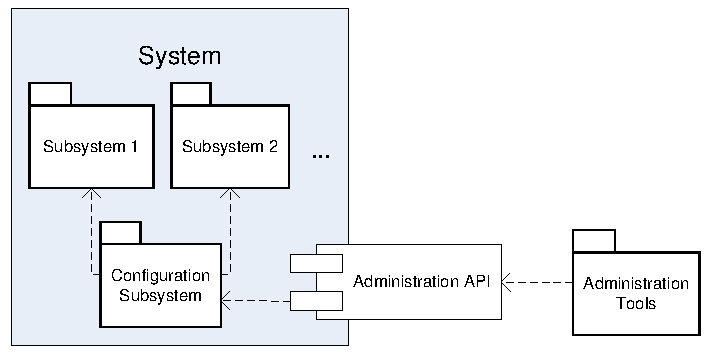
\includegraphics{patterns/provideAPIDiagram-01.pdf}
\caption{Main solution structure of PROVIDE AN ADMINISTRATION API}
\label{fig:provideAPIDiagram-01}
\end{figure}

If the administration API should not be publicly available due to security reasons, a {\sc Proxy} \cite{Buschmann1996} could be used to adequately address this issue. Figure \ref{fig:provideAPIDiagram-02} shows the main design. The protection proxy needs to include some mechanism for authentication and authorization of the requester. These can be implemented making use of e.g. patterns {\sc Adapter} \cite{Gamma95} because this pattern can influence the visibility of the administration API with respect to authentication and authorization of the requester.
%(TODO) @Christian: is dit wat je voor ogen hebt?.

\begin{figure}[h]
\centering
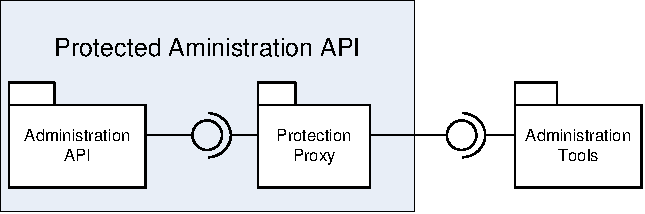
\includegraphics{patterns/provideAPIDiagram-02.pdf}
\caption{An administration API including a protection proxy for security reasons}
\label{fig:provideAPIDiagram-02}
\end{figure}

In certain cases the implementation language of the system and that of the administration API are different. Main reason for this could be that the administration API is required to be provided in a specific scripting language that suits the administrators' tasks best. In that case the administration API subsystem also becomes a specific kind of an {\sc Adapter} \cite{Gamma95} between these two implementation languages.

The problem of different platforms used for the system and in the administration environment can be minimized by making use of cross-platform scripting languages like Python, Ruby or TCL. This is also a certain advantage above graphical administration interfaces, as it removes the platform-specific issues caused by the GUI technologies. In combination with such a cross-platform scripting language this pattern shows its real strength as one can uniformly approach the administration API on any given platform.

Ideally, any changes in the system itself do not lead to changes in the administration API. However, if also functionality of the system regarding its configuration is changing, then also the API likely needs to be changed. The tools of the administrators are dependent on the API both syntactically and semantically in varying degrees. Unfortunately are both dependency types interrelated: the less syntactic the dependency is, the higher it is semantically and vice versa. One criterion that can be used for determining if the API should decrease the syntactic or the semantic dependencies is how easy it is to adapt the connection to the API on either syntactic and semantic level. If the interfaces are easy to adapt on both sides, then one should prefer more syntactically dependent interfaces that explicitly contain the semantic information in the naming of the methods and parameters. If the interfaces are not easy to adapt, then the syntactical dependencies should be low by using more generic interfaces that merely require different parameter contents but no interface adaptations.  

%TODO: some stuff on documentation of the API.




\textit{One possibility of implementing this administrative API in the Java programming language are Java Management Extensions\footnote{\url{http://www.oracle.com/technetwork/java/javase/tech/javamanagement-140525.html}} (JMX). }
%
%\begin{center}
%\ding{118} \ding{118} \ding{118} 
%\end{center}
%
%\textit{Rationale?}\\
%%Using this pattern will make the life of a system administrator more pleasant, especially in cross-platform situations, as it removes the platform-specific issues caused by a graphical administration interface. In combination with a cross-platform scripting language (e.g. Python, Ruby, TCL) this pattern shows its real strength as one can uniformly approach the administration API on any given platform.
%

\newpage
\section*{SINGLE FILE LOCATION AND STRUCTURE}
% \parskip=0.3em
\textit{Context:}\\
Files are an established mechanism used by applications to store and retrieve configuration, libraries, state, data etc. Newly developed applications tend to use files in their own unique manner and store files in various locations. This may lead to having files that are dispersed over different folders or hidden in system-folders of the Operating System. System administrators  want to be able to perform version control on the files.
\begin{center}
\ding{118} \ding{118} \ding{118}
\end{center}

\textit{Problem and forces:\\}
\textbf{Having dispersed files causes system administrators to have difficulty in finding the files necessary for their tasks during the life cycle of an application.}\\

%forces
\begin{itemize}
\item Distributed Applications.\\
Many applications consist of different subsystems, which often require  subsystem-specific administration tasks. These subsystems are in many cases developed by different teams, resulting in dispersed groups of similar artifacts for each subsystem. This situation is well suited for developers as they can work in parallel. During deploy or system administration activities this can be a burden because of the way they have to look in different locations.
\item Hard-coded Locations.\\
It happens often that developers put the location of the configuration files in source code and provide no parameters or interface to influence this location. This means the path can only be changed by building and deploying a new version of the application. Running multiple instances of a program on a machine with different parameters is effectively blocked by this approach. Additionally it can pose security risks if the file location is in a privileged location such as \verb|C:\Program Files| for Windows based systems.


\item Pollution.\\
When a file of a module isn't used anymore it will easily remain in disuse and get overlooked which causes pollution of your hard disk.\\
\end{itemize}

\begin{center}
\ding{118} \ding{118} \ding{118} 
\end{center}

\textbf{Therefore: Put all related files in a folder hierarchy relative to one location on a file system or repository. Make the path of this location configurable.}\\

\textit{Solution description:}\\
Analyze the files and folders of the application, group the files  that logically belong together and should be at the same location in a folder e.g.: the binaries of a system, the configuration files and the data files. In the case of log files one should first consider to use {\sc Centralized System Logging}.

Ideally it should be a structure that is re-used across applications (see figure \ref{fig:singleFileLocationDiagram-01}) that are installed on the same server. This provides consistency for the system administrator, but also might help to overcome possible redundancies of files (e.g. keeping track of the language used). It furthermore serves as a clear guideline for the developers and could also be included in a reference architecture.

For reading the contents of configuration files {\sc Property Loader} and related patterns \cite{Wellhausen2010} can be used. 

If an application is deployed several times on a server it may be necessary to include the name of each specific application instances in the path on the file system. E.g. use \verb|/somewhere/theapp/internal| and \verb|/somewhere/theapp/external| if an application instance is deployed once for internal users and once for external users on the same server. This will separate the files for each application deployment. A common practice in these cases is to a symbolic link to share common files across all deployed instances. 
\begin{figure}[h]
\centering
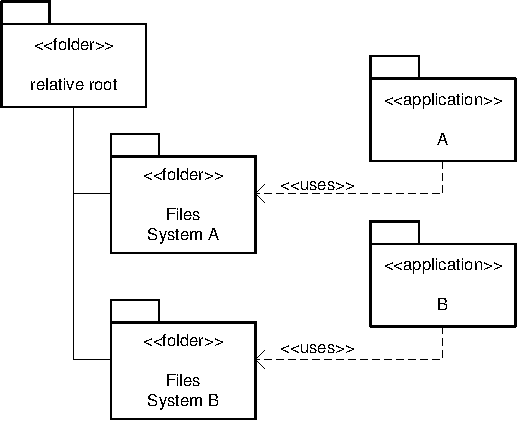
\includegraphics{patterns/singleFileLocationDiagram-01.pdf}
\caption{The hierarchical file structure}
\label{fig:singleFileLocationDiagram-01}
\end{figure}

The applications that do file access should not use the native File IO Libraries but should use a {\sc Facade} \cite{Gamma95} for accessing files (see figure \ref{fig:singleFileLocationDiagram-02}). This {\sc Facade} provides the basic file IO functionality and prohibits absolute path access. The {\sc Facade} is using a configurable absolute path that is the root of all file access. The relative paths branch from that root path.  This is best enforced in combination with a build server that checks which libraries are used from source code. The build should break when native File IO Libraries are used instead of the library that provides the {\sc Facade}. 

If the folder structure to be used for applications is standardized across a development group, developers find it easier to navigate across an application and find the right files and folders. This can also be supported by providing skeleton solution or projects structures within the development environments such as Eclipse or Microsoft Visual Studio.

\begin{figure}[h!]
\centering
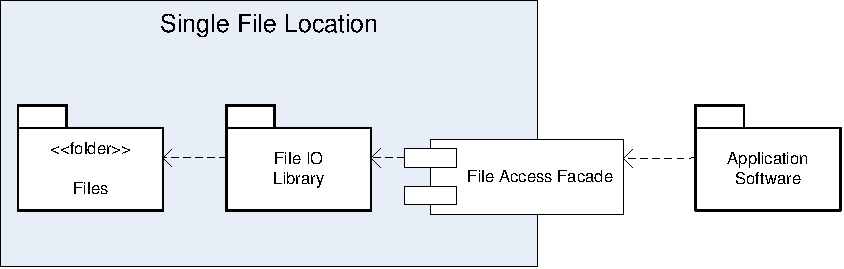
\includegraphics{patterns/singleFileLocationDiagram-02.pdf}
\caption{Main solution structure for file access using SINGLE FILE LOCATION}
\label{fig:singleFileLocationDiagram-02}
\end{figure} 

\begin{center}
\ding{118} \ding{118} \ding{118} 
\end{center}

\textit{Rationale:}\\
When not using this pattern the files of applications will be dispersed over several distinct locations which makes it hard to maintain the application.

Using SINGLE FILE LOCATION AND STRUCTURE is also more secure as this blocks access to other parts of the filesystem on the server as the implemented {\sc Facade} blocks access outside the root location. It is somewhat similar to a jailshell which is widely used to constrain linux users within their homefolder.

\textit{A nice example of the structure of SINGLE FILE LOCATION AND STRUCTURE 
 without a {\sc Facade} is for instance found in the way applications based on the Ruby on Rails (RoR) framework \cite{Rails} are structured. Every project starts with a pre-defined folder and file structure. RoR organizes all models, view and controller related logic in model, view and controller folders. Alle configuration settings are stored in a configuration folder and the Development, Test and Production stages related settings are stored in subfolder of the configuration folder. The framework provide internal relative paths to these folders so application can be stored in any location as long as the structure within the application folder remains the same.}

\textit{Another example is the Filesystem Hierarchy Standard \cite{FHS}. FHS defines the directory structure and directory contents in Unix and Unix-like operating systems, maintained by the Linux Foundation. Most Linux distributions follow the Filesystem Hierarchy Standard and maintain FHS compliance. Similar constructs are found in how OSX organizes applications and application data in file hierarchy}

\newpage
\section*{BUILT-IN SYSTEM LOGGING}

The application needs to provide the ability of logging certain events or actions by using the built in system logging of a platform. 

\begin{center}
\ding{118} \ding{118} \ding{118}
\end{center}

\textbf{Having a variety of logging formats and log-file locations makes it hard to monitor the state of a whole enterprise, including all running applications.}\\

\textit{Format Variety.} A high variety of logging formats increases the complexity of integrating the information held within those several log files. It becomes a burden to nullify the different lay-outs of these log files.\\ 

\textit{Location Variety.} When having a variety of log file locations the dispersion of those locations makes it difficult to gather those files to one stack.\\

\textit{Information Granularity.} Not only the formats might be varying, but also the granularity of information. This makes it hard to monitor all applications in a consistent way or to integrate the information in a consistent way for other statistical purposes like e.g. root cause analysis\footnote{\url{http://en.wikipedia.org/wiki/Root_cause_analysis}}.

\begin{center}
\ding{118} \ding{118} \ding{118} 
\end{center}

\textbf{Therefore: Use the built-in system logging mechanism whenever possible. If it is not possible, then define a standard format to be used by all systems and implement your own logger.}\\

Many monitoring tools use the system built-in logging mechanisms. The connection between these is well defined and proven. It is therefore of help for the system administrators if these built-in logging mechanisms are used by all applications, as this allows the administrators to make use of existing tools (e.g. Nagios\footnote{\url{http://www.nagios.org/}} or HP OpenView) that collect, centralize, and search the logs \cite{Limoncelli2011a}.

The built-in system logging mechanisms take care of the log file location problem. They also prescribe the format, thereby forcing the developers, but also supporting them, to make consistent use of logging on the appropriate granularity.

It is also a lot easier to automatically generate incidents from specific defined events from the built-in system log for an IT service management (ITSM) tool. This ITSM tool can be configured to forward the automatically generated incidents directly, without human intervention, to the second line specialists. This way incidents are more easily solved without less human intervention, saving valuable time of the system administrators.

Of course logging in many cases has to be activated from within the system, so developers often have to explicitly program it into the system. But using the built-in logging mechanism alone does not ensure that the developers also make use of logging when it is appropriate. To address this issue guidelines could be defined and used by the developers for including logging in the system. 

If it is not possible to use the built-in system logging, e.g. because of different operating systems being used, then develop your own {\sc Diagnostic Logger} \cite{Harrison2001} and define a standard for your system landscape that works good in combination with the administration tools being used. Use the properties of built-in system logging mechanisms as basis for the requirements of your own logging mechanism. The most important point hereby is that this mechanism can be connected to the ITSM tools used by the system administrators. Ensure that this standard system is used for logging. This approach can be combined with {\sc Single File Location}.

Some requirements a good log should met to be valuable are:
\begin{itemize}
	\item Log actions before they happen.
	\item Mind the file size if logs should be copied or archived.
	\item Split messages into different files depending on intended audience/way of using.
\end{itemize}


To Do: \\
For implementing a (system) logging facility one can make use of the  pattern {\sc Memento} \cite{Gamma95} which is ... Writing to a log entry is best done with the pattern {\sc Command} \cite{Gamma95} and the logger itself is best implemented with pattern {\sc Factory} \cite{Gamma95}, which creates Mementos for logged events.

Add: Figure(s)

%\begin{figure}[h]
%\centering
%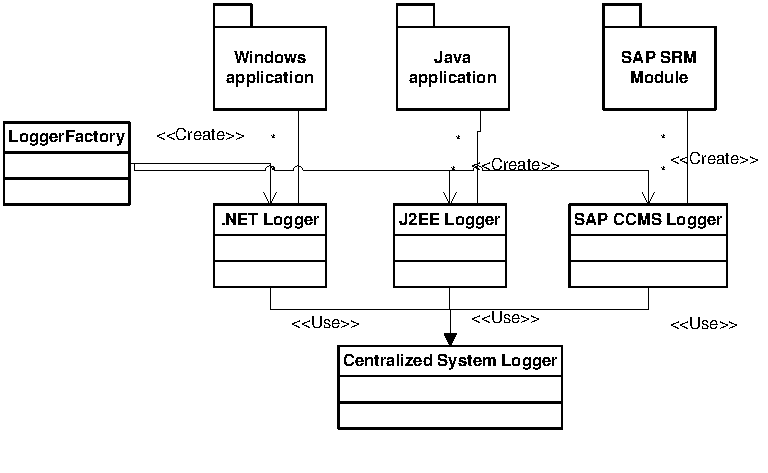
\includegraphics{patterns/systemLoggingDiagram.pdf}
%\caption{Main solution structure of BUILT-IN SYSTEM LOGGING}
%\label{fig:systemLogging}
%\end{figure}
%
%See figure \ref{fig:systemLogging}.

%\begin{center}
%\ding{118} \ding{118} \ding{118} 
%\end{center}






%\newpage
\section*{CENTRALIZED IDENTITY MANAGEMENT}
also known as: IDENTITY MANAGEMENT BUS.

The system makes use of user identities which need to be managed. 

\begin{center}
\ding{118} \ding{118} \ding{118}
\end{center}

\textbf{Decentralized user identity management means a lot of extra work as identities have to be managed on many different places and it is hard to get a centralized overview of all existing or available identities. This also makes role management much more complex.}\\

\textit{Separation of Duties.} Especially when Separation of Duties (SoD) is a concern such as within financial environments it is important for organizations to be able to show to e.g. an EDP auditor that all regulations are fulfilled.

\begin{center}
\ding{118} \ding{118} \ding{118} 
\end{center}

\textbf{Therefore: Make use of a centralized identity management system if this is available.}\\

This solution has several advantages: if the centralized identity management system (CIM) is also connected to the human resources system (HRM)-system, it is easier to revoke certain grants due to retirements etc. Also user roles could be (automatically) inferred from function profiles in the HRM system.

%Relation with possible {\sc Centralized Role Management} pattern and {\sc Role Based Access Control (RBAC)} and at a lower level {\sc Access Control List (ACL)}?

When no centralized identity management system is available a lot of organizations make use of something like Active Directory Services (ADS). Mostly in these cases where ADS is used this isn't connected to a HR system whereby the events or triggers for the HR processes placing in, leave service, function change or department change are missed in the ADS. This causes an increase in maintenance activities to take care of pollution of the ADS.

%TODO: describe an alternative solution if no centralized identity management system is available (RB: dit is juist het probleem wat hiermee opgelost dient te worden. Heel veel organisaties gebruiken dan alleen het ADS (Active Directory Services) als identity source, maar dat is meestal niet gekoppeld aan het personeelssysteem, waardoor de events/triggers voor bv. in-/uitdienst, functiewijziging of afdelingswijziging gemist worden en de situatie vanuit beheeroogpunt lastig beheerbaar wordt).

\begin{center}
\ding{118} \ding{118} \ding{118} 
\end{center}

There is an urgent need within medium to large organizations to centralize role based access information. Several applications have role based access information. This dispersion of information leads to a high maintenance sensitivity. Which demands a high level of deployment. Therefore the dispersion of information needs to be centralized within a solution according to this pattern.
% Many organisations have several identity sources, e.g. HR-system, Active Directory, access management systems (physical). --> mochten we ook metadirectories willen toelichten, maar voor nu laat ik het even buiten beschouwing.
%\newpage
\section*{MULTI-TENANT APPLICATION}

%Het Multi-tenancy patroon is een patroon wat op meerdere niveaus toegpast kan worden: data, software, hardware. In het kader van dit artikel zal alleen de softwarekant genoemd worden, omdat deze van invloed is op het resourceverbruik van servers binnen een rekencentrum en om het resourceverbruik omlaag te krijgen.
% Er is best wel wat literatuur over multi-tenancy te vinden zodoende heb ik nog niet alles kunnen lezen. In het onderzoekssemester (Semester 7 - blok 1 & 2) ga ik een onderzoeksgroep bij de gemeente Utrecht begeleiden.

A multi-tenant application is a shared solution (i.e. HRM) used by different tenants ((client) organizations, departments). It is a single application with scalable resources to meet the performance demands of tenants. 

\begin{center}
\ding{118} \ding{118} \ding{118}
\end{center}

\textbf{Many companies are looking for a scalable architecture to deal with burst loads or for an approach for sharing. Virtualizing your hardware seemed one solution but isn't realy scalable in both directions (upwards and downwards)}\\

%\textit{Elastic computing.} ...

\begin{center}
\ding{118} \ding{118} \ding{118} 
\end{center}

\textbf{Therefore: Make use of multi-tenant applications to reduce hardware investments or to outsource one's software and hardware to a SaaS/PaaS-provider.}\\

This solution has several advantages: Combining virtualization, elasticity and multi-tenancy results in optimized usage of data center
resources as it means CPU, memory and network resources are maximally deployed.

%Relation with possible {\sc Virtualization} pattern and {\sc Elasticity}?

When no multi-tenancy is used a lot of organizations make use of virtualization and/or elasticity.

%TODO: describe an alternative solution if no multi-tenancy is available (RB: dit is juist het probleem wat hiermee opgelost dient te worden. Heel veel organisaties gebruiken dan alleen virtualisatie of elasticiteit in bv. een vorm als Amazon EC2 (Elastic Compute Cloud)) waarmee echte schaalbaarheid lastig te verkrijgen is. 

\begin{center}
\ding{118} \ding{118} \ding{118} 
\end{center}

Besides above mentioned advantages multitenant applications are typically required to provide a high degree of customization to support each target organization's needs. Customization typically includes the following aspects:
\begin{itemize}
  \item Branding: allowing each organization to customize the look-and-feel of the application to match their corporate branding (often referred to as a distinct "skin").
	\item Workflow: accommodating differences in workflow to be used by a wide range of potential customers.
	\item Extensions to the data model: supporting an extensible data model to give customers the ability to customize the data elements managed by the application to meet their specific needs.
	\item Access control: letting each client organization independently customize access rights and restrictions for each user.\footnote{\url{http://en.wikipedia.org/wiki/Multitenancy}}
\end{itemize}


\section{Conclusion} 

%Rebecca: Ending conclusion/ much overlap with introduction (Eigenaar: Roland)

%Unknown3: Intro? Jah?
%Leo: Not really a conclusion
%Leo: Future work: Too detailed; do not name future patterns
In the article \textit{A plea from sysadmins to software vendors: 10 Do's and Don'ts} by Thomas Limoncelli \cite{Limoncelli2011a}, system administrators collected a basic list of do's and dont's for software vendors in order to make the life of the system administrators more easy. 

This paper aims at influencing the software architects and the software architecture by providing patterns for software architecture that are endorsed by system administrators.

%There have been several initiatives to describe patterns from the perspective of a system administrator, but these are mainly focused on infrastructure and middleware. Examples of these initiatives are: 
%\begin{itemize}
%	\item Open Infrastructure Architecture repository (OIAr)\footnote{\url{http://www.infra-repository.org/oiar/index.php/Main_Page}} 
%	\item Enterprise Integration Patterns\footnote{\url{http://www.eaipatterns.com/}}
%\end{itemize}

Both approaches --- software architecture patterns for realizing the above described quality attributes and patterns that support the work of system administrators --- don't touch some important aspects of the intersection of software architecture and system administration. Therefore we want
%Leo: W.r.t. want: Presearch on the application of the 3 patterns?
to introduce a set of patterns which bridges this gap, based on the needs of the system administrators. 

The problems that are cited in the aforementioned article have been experienced within daily system administration practice. 

Further patterns we want to work on are {\sc Centralized Identity Management} and {\sc Multi-tenancy}.
% Leo: Do not describe the patterns
% {\sc Centralized Identity Management} is interesting because there is an urgent need within medium to large organizations to centralize role based access information. The importance of {\sc Multi-tenancy} lies in the fact that it is a shared solution (i.e. HRM) used by different tenants ((client) organizations, departments). E.g. many municipalities have dispersed departments with their own system owners but want to share resources without creating security leaks. Multi-tenancy is an option to reach this goal of sharing resources.

With this starting point for a repository of this kind of patterns we want to give ideas to software architects and application developers on how to improve their applications from a system administration viewpoint. Beside these patterns we want to bridge the gap between system administrators and the software architects of the software which needs to be administered by these system administrators. \\
We think it is interesting to look for a specialized modelling language like SysML \cite{SysML} to describe these patterns in the future. 

\section{Acknowledgements}
We wish to express many thanks to our shepherd Eduardo Guerra for all his useful comments and feedback. Furthermore the feedback given by the participants of the writers' workshop at the PLoP'13 conference helped a lot to improve this work.

%\bibliographystyle{plain}
% Referentie naar Poort en Vliet dienen nog uit de bibliografie verwijderd te worden.
\bibliographystyle{acmlarge}
\bibliography{ArchitecturePatterns}
\end{document}
